% 原书第191—195页；9.5.5、9.5.6。
\subsection{检测低复杂度混杂因子}
这里介绍Janzing et al.［2011］提出的两种方法，用于推断两个观测变量$X,Y$之间的路径，是否经过某个仅取少量值的中间变量，见图9.10。具体设定如下：$X$通过一个在$Y$处带有箭头的DAG与$Y$存在因果联系。问题是，$X,Y$之间的路径中，是否存在一个仅取少量值的中间变量$U$。这里，连接$X$与$U$的箭头方向并不重要；不过，这些方法的典型应用，是在混杂路径经过这样一个简单变量$U$时检测混杂。
\begin{figure}[htbp]
\centering
\begin{tikzpicture}[causal,x=1.4cm,y=1cm]
 \node[vtx] (ch09f10a-x) at (0,0) {$X$};
 \node[latent] (ch09f10a-u) at (1,0) {$U$};
 \node[vtx] (ch09f10a-y) at (2,0) {$Y$};
 \node[vtx] (ch09f10b-x) at (4,0) {$X$};
 \node[latent] (ch09f10b-u) at (5,0) {$U$};
 \node[vtx] (ch09f10b-y) at (6,0) {$Y$};
 \draw[ed] (ch09f10a-u)--(ch09f10a-x);
 \draw[ed] (ch09f10a-u)--(ch09f10a-y);
 \draw[ed] (ch09f10b-x)--(ch09f10b-u);
 \draw[ed] (ch09f10b-u)--(ch09f10b-y);
\end{tikzpicture}
\caption{检测低复杂度中间变量：如果$X$与$Y$之间的路径被一个只取少量值的变量$U$阻断，$P_{Y\mid X}$往往会呈现一些典型性质，作为$U$的“指纹”。}
\end{figure}


例如，Janzing et al.［2011］考虑用两个二值变量$X,U$描述动物或植物的遗传变异，即单核苷酸多态性，再用变量$Y$描述某个表型。如果$X$与$Y$之间的统计相依，完全源于$U$影响$Y$、而$U$在统计上与$X$有关，那么$U$就发挥这种中间变量的作用。这里，$U$与$X$都不是对方的原因，而是存在“族群”等同时影响二者的变量。因此，$U$本身不是共同原因，但位于混杂路径上。

检测这类混杂的基本思想，是$U$会以一种特征性的方式改变条件分布$P_{Y\mid X}$。为讨论这一点，先定义一类条件分布；随后将说明，只有当$X,Y$之间的路径不经过上述$U$时，这类条件分布才通常会出现。

\begin{definition}[两两纯条件分布]
若对任意两个$x_1,x_2\in\mathcal X$，都满足如下条件，则称条件分布$P_{Y\mid X}$具有\textbf{两两纯性（pairwise purity）}：不存在$\lambda<0$或$\lambda>1$，使
\begin{equation}
 \lambda P_{Y\mid X=x_1}+(1-\lambda)P_{Y\mid X=x_2}
 \tag{9.19}
\end{equation}
是一个概率分布。
\end{definition}

为理解定义9.6，注意，当$\lambda\in[0,1]$时，式(9.19)总是概率分布，因为此时它是两个分布的凸组合。另一方面，如果$\lambda\notin[0,1]$，式(9.19)可能不再是非负测度。考虑$Y$只取有限多个值$\mathcal Y:=\{y_1,\ldots,y_k\}$的情况：$Y$的分布空间是一个单纯形，其$k$个顶点分别为集中在$y_1,\ldots,y_k$上的点质量。图9.11展示了$k=3$的情况，此时$\mathcal Y$上的概率分布空间是一个三角形。
\begin{figure}[htbp]
\centering
\begin{minipage}[t]{.47\linewidth}
\centering
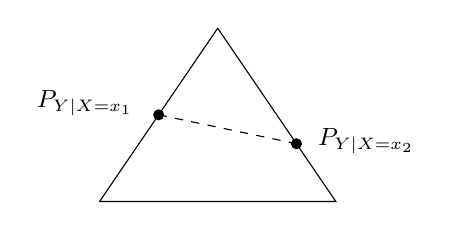
\begin{tikzpicture}[x=1cm,y=1cm]
 \draw (0,0)--(1.5,2.2)--(3,0)--cycle;
 \draw[dashed] (.75,1.1)--(2.5,.733333);
 \fill (.75,1.1) circle[radius=2pt];
 \fill (2.5,.733333) circle[radius=2pt];
 \node[left,font=\small] at (.55,1.25) {$P_{Y\mid X=x_1}$};
 \node[right,font=\small] at (2.65,.77) {$P_{Y\mid X=x_2}$};
\end{tikzpicture}
\par\small (a) 纯条件分布的示例：延长连接$P_{Y\mid X=x_1}$与$P_{Y\mid X=x_2}$的线段，就会离开概率分布单纯形。
\end{minipage}\hfill
\begin{minipage}[t]{.47\linewidth}
\centering
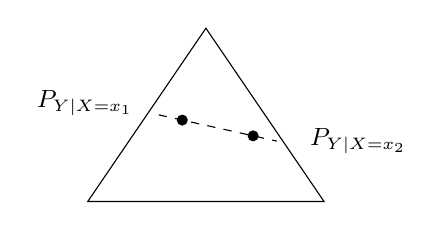
\begin{tikzpicture}[x=1cm,y=1cm]
 \draw (0,0)--(1.5,2.2)--(3,0)--cycle;
 \draw[dashed] (.9,1.1)--(2.4,.766667);
 \fill (1.2,1.033333) circle[radius=2pt];
 \fill (2.1,.833333) circle[radius=2pt];
 \node[left,font=\small] at (.7,1.25) {$P_{Y\mid X=x_1}$};
 \node[right,font=\small] at (2.7,.77) {$P_{Y\mid X=x_2}$};
\end{tikzpicture}
\par\small (b) 非纯条件分布的示例：连接$P_{Y\mid X=x_1}$与$P_{Y\mid X=x_2}$的线段，可以稍作延长而不离开单纯形。
\end{minipage}
\caption{纯条件分布与非纯条件分布的可视化。}
\end{figure}


图9.11(a)给出一个纯条件分布的例子：延长$P_{Y\mid X=x_1}$与$P_{Y\mid X=x_2}$之间的连线，就会离开三角形；而在图9.11(b)中，可以在分布空间内继续延长这条连线。不过，图9.12说明，纯性强于“各点$P_{Y\mid X=x}$位于单纯形内部”这一条件：这里，两点位于三角形的边上，却仍允许在三角形内延长连线。\chninenote{定义9.6及下方密度判据中的“任意两个$x_1,x_2$”，应限定为不同取值；否则取$x_1=x_2$时不可能满足纯性。另一个原文措辞问题是“位于单纯形内部”：图9.12实际说明的是，仅要求各点位于单纯形边界仍不足以保证纯性。主文保留原句含义，并据图例作此澄清。}
\begin{figure}[htbp]
\centering
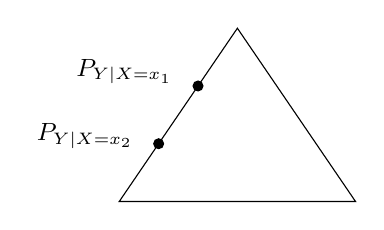
\begin{tikzpicture}[x=1cm,y=1cm]
 \draw (0,0)--(1.5,2.2)--(3,0)--cycle;
 \fill (1,1.466667) circle[radius=2pt];
 \fill (.5,.733333) circle[radius=2pt];
 \node[left,font=\small] at (.8,1.65) {$P_{Y\mid X=x_1}$};
 \node[left,font=\small] at (.3,.83) {$P_{Y\mid X=x_2}$};
\end{tikzpicture}
\caption{非纯条件分布的另一个例子：连接$P_{Y\mid X=x_1}$与$P_{Y\mid X=x_2}$的线段，可以延长而不离开单纯形。}
\end{figure}


若$P_{Y\mid X}$具有密度$(x,y)\mapsto p(y\mid x)$，则可以用下面这个直观条件定义纯性：
\[
 \inf_{y\in\mathcal Y}\frac{p(y\mid x_1)}{p(y\mid x_2)}=0,
 \qquad\forall x_1,x_2\in\mathcal X.
\]
自然界中对应于$X\to Y$的因果条件分布，究竟在多大程度上具有纯性，仍有待未来研究。这里给出一类有意义的纯条件分布：若$P_{Y\mid X}$可以由函数$f_Y$为双射的加性噪声模型表示［Janzing et al., 2011，引理4］，且噪声密度满足某个衰减条件，则$P_{Y\mid X}$具有两两纯性。

下面的结果说明，纯条件分布强烈提示：$X,Y$之间的因果路径没有经过一个仅取少量值的中间变量。
\begin{theorem}[严格正的条件分布与非纯性]
假设存在变量$U$使$X\indep Y\mid U$。进一步假设$U$的值域$\mathcal U$有限，且对所有$u\in\mathcal U$及使$P_{Y\mid X=x}$有定义的$x$，条件密度$p(u\mid x)$都严格为正。那么，$P_{Y\mid X}$不具有两两纯性。
\end{theorem}
\begin{proof}
容易看出，条件分布$P_{U\mid X}$不具有两两纯性，因为对所有使$P_{Y\mid X=x_i}$有定义的$x_1,x_2$，都有
\[
 \inf_{u\in\mathcal U}\frac{p(u\mid x_1)}{p(u\mid x_2)}\ne0.
\]
又因为$p(y\mid x)=\sum_u p(y\mid u)p(u\mid x)$，条件分布$P_{Y\mid X}$是$P_{Y\mid U}$与$P_{U\mid X}$的复合。既然$P_{U\mid X}$不具有纯性，$P_{Y\mid X}$也不具有纯性［见Janzing et al., 2011，引理8］。
\end{proof}

虽然这一定理适用于所有有限值变量，但如果$U$只取少量值，关于条件分布$P_{U\mid X}$严格为正的第二项假设就合理得多。否则，可能存在一些$u$，使$p(u\mid x)$非常接近$0$，以至于$P_{Y\mid X}$\emph{几乎}具有纯性。

下面的例子可以直观展示，中间节点通常如何破坏纯性。假设$U,X$均为二值变量，并在$u=x$时满足$p(u\mid x)=1-\varepsilon$。于是
\[
\begin{aligned}
 P_{Y\mid X=0}
 &=P(U=0\mid X=0)P_{Y\mid U=0}
  +P(U=1\mid X=0)P_{Y\mid U=1}\\
 &=(1-\varepsilon)P_{Y\mid U=0}+\varepsilon P_{Y\mid U=1}.
\end{aligned}
\]
因此，$P_{Y\mid X=0}$位于连接$P_{Y\mid U=0}$与$P_{Y\mid U=1}$的线段内部，$P_{Y\mid X=1}$也一样。所以$P_{Y\mid X}$不具有纯性。

中间变量还可能以另一种方式，在分布$P_{X,Y}$中留下特征性“指纹”。我们利用条件分布的下列性质表述这一点［Allman et al., 2009；Janzing et al., 2011］。
\begin{definition}[条件分布的秩]
$P_{Y\mid X}$的\textbf{秩（rank）}，是测度空间中所有向量$P_{Y\mid X\in A}$所张成向量空间的维数，其中$A$遍历$X$值域中概率非零的全部可测子集。
\end{definition}

不过，Janzing et al.［2011］没有提供估计秩的算法。若$Y$的值域有限，则$P_{Y\mid X}$定义一个随机矩阵，其秩与$P_{Y\mid X}$的秩相同。下面的结果是一个简单的观察［Allman et al., 2009］。
\begin{theorem}[秩与$U$的值域]
若$X\indep Y\mid U$且$U$取$k$个值，则$P_{Y\mid X}$的秩至多为$k$。
\end{theorem}

容易证明，在定理9.9的条件下，$P_{X,Y}$可以分解为$k$个乘积分布的混合。这一观察可以推广到多元情形：只要存在一个取$k$个值的变量$U$，使$X_1,\ldots,X_d$在给定$U$后相互独立，那么$P_{X_1,\ldots,X_d}$就能分解为$d$个乘积分布的混合。\chninenote{本句原印为“$d$个乘积分布”，其中$d$是观测变量数；混合项数应为$U$的取值数$k$，每个乘积分布含$d$个因子。主文保留原计数。}Sgouritsa et al.［2013］与Levine et al.［2011］描述了寻找这种分解的方法，目标是通过识别乘积分布，检测“混杂因子”$U$。
\FloatBarrier

\subsection{不同环境}
第7.1.6节与第7.2.5节介绍的不变因果预测方法，可以修改后用于处理潜变量［Peters et al., 2016，第5.2节］，前提是潜变量不受干预影响。此外，Rothenhäusler et al.［2015，“backShift”］考察了线性结构因果模型这一特例。

假设我们在不同环境$e\in\mathcal E$中，观测由$d$个随机变量构成的向量$\mathbf X^e$。这些环境由未知的\textbf{移位变量（shift variable）}$\mathbf C^e=(C_1^e,\ldots,C_d^e)$产生；要求其各分量彼此独立，并与噪声变量独立。也就是说，对每个环境$e$，都有
\[
 \mathbf X^e=\mathbf B\mathbf X^e+\mathbf C^e+\mathbf N^e,
\]
其中$\mathbf N^e$的分布不依赖于$e$。允许噪声向量的不同分量之间存在非零协方差，就可以纳入潜变量。此时仍有
\[
 (I-\mathbf B)\Sigma_{\mathbf X,e}(I-\mathbf B)^T
 =\Sigma_{\mathbf C,e}+\Sigma_{\mathbf N},
\]
其中$\Sigma_{\mathbf X,e}$、$\Sigma_{\mathbf C,e}$和$\Sigma_{\mathbf N}$分别为$\mathbf X^e$、$\mathbf C^e$与$\mathbf N^e$的协方差矩阵。因此，
\begin{equation}
 (I-\mathbf B)\bigl(\Sigma_{\mathbf X,e}-\Sigma_{\mathbf X,f}\bigr)(I-\mathbf B)^T
 =\Sigma_{\mathbf C,e}-\Sigma_{\mathbf C,f}.
 \tag{9.20}
\end{equation}
注意，对每个环境$e$，都可以将其余环境合并，得到“环境”$f$。根据假设，无论如何选择$e,f$，式(9.20)右侧都是对角矩阵，因此可以通过对$\Sigma_{\mathbf X,e}-\Sigma_{\mathbf X,f}$进行\textbf{联合对角化（joint diagonalization）}，重建因果结构$\mathbf B$。如果至少有三个环境，该过程就能在一些较弱假设下识别$\mathbf B$［Rothenhäusler et al., 2015，定理1］。

最后这个例子说明，通过在不同环境之间施加规律性条件，例如线性模型与独立移位干预，即使存在潜变量，也能重建底层因果结构。
\FloatBarrier
